\section{Appendix-C Distributions and formula's}


\subsection{Soil load on the quay wall}

The soil behind the wall is modelled as a triangular lateral earth pressure,
$\sigma_h(z) = K\,\gamma_s\,z$, which reaches $K\gamma_s H$ at the base of the
retained height $H$. The resultant soil force per metre of wall and its
moment about the base are
\begin{align}
  F_s &= \int_0^H K\,\gamma_s\,z\,\mathrm{d}z = \tfrac{1}{2}\,K\,\gamma_s\,H^2
        && [\mathrm{kN/m}], \label{eq:soil_force}\\
  S   &= F_s\,\frac{H}{3} = \tfrac{1}{6}\,K\,\gamma_s\,H^3
        && [\mathrm{kNm/m}], \label{eq:soil_load}
\end{align}
where $K$ is the lateral earth pressure coefficient [--], $\gamma_s$ the unit
weight of the soil [kN/m$^3$] and $H$ the retained height [m]. The resultant
force $F_s$ acts at $H/3$ above the base.

$K$ and $\gamma_s$ are treated as independent random variables, with one set
of parameters per soil type (Table~\ref{tab:soil_distributions}). $K$ is
lognormal, with $\sigma_{\ln} = \sqrt{\ln(1+V_K^2)}$ and
$\mu_{\ln} = \ln\mu_K - \tfrac{1}{2}\sigma_{\ln}^2$, so that its mean and
coefficient of variation match the table. $\gamma_s$ is normal, and
$\kappa_{f,0}$ is deterministic.

\begin{table}[htbp]
  \centering
  \caption{Probabilistic soil parameters per soil type
           ($\mu$ = mean, $V$ = coefficient of variation).}
  \label{tab:soil_distributions}
  \begin{tabular}{lcccccc}
    \toprule
    & \multicolumn{2}{c}{$K$ [--], lognormal}
    & \multicolumn{2}{c}{$\gamma_s$ [kN/m$^3$], normal}
    & \multicolumn{2}{c}{$\kappa_{f,0}$ [--], deterministic} \\
    \cmidrule(lr){2-3} \cmidrule(lr){4-5} \cmidrule(lr){6-7}
    Soil type & $\mu$ & $V$ & $\mu$ & $V$ & shallow & piles \\
    \midrule
    Soft clay / peat & 0.60 & 0.20 & 15.0 & 0.05 & 0.80 & 1.10 \\
    Sand             & 0.35 & 0.20 & 18.0 & 0.05 & 1.00 & 1.20 \\
    Mixed / layered  & 0.45 & 0.25 & 16.5 & 0.06 & 0.90 & 1.15 \\
    \bottomrule
  \end{tabular}
\end{table}

Because $K$ and $\gamma_s$ are independent, the mean soil load is
$\mu_S = \tfrac{1}{6}\,\mu_K\,\mu_{\gamma}\,H^3$ and its coefficient of
variation is $V_S = \sqrt{(1+V_K^2)(1+V_\gamma^2) - 1}$, independent of $H$.
This gives $V_S = 0.21$ for soft clay / peat and sand and $V_S = 0.26$ for
mixed / layered soil; the scatter comes almost entirely from $K$, since
$V_\gamma \leq 0.06$. A Monte Carlo simulation with $10^5$ draws per soil
type confirms this. At $H = 3$\,m the mean soil load is 40.5\,kNm/m for soft
clay / peat, 33.4\,kNm/m for mixed / layered soil and 28.4\,kNm/m for sand,
with 5--95\% ranges of 28.4--55.5, 21.3--49.1 and 19.9--38.8\,kNm/m. Since
$S \propto H^3$, doubling the retained height increases the soil load by a
factor of eight.


\begin{figure}[ht]
    \centering
    \begin{subfigure}[b]{0.40\linewidth}
        \centering
        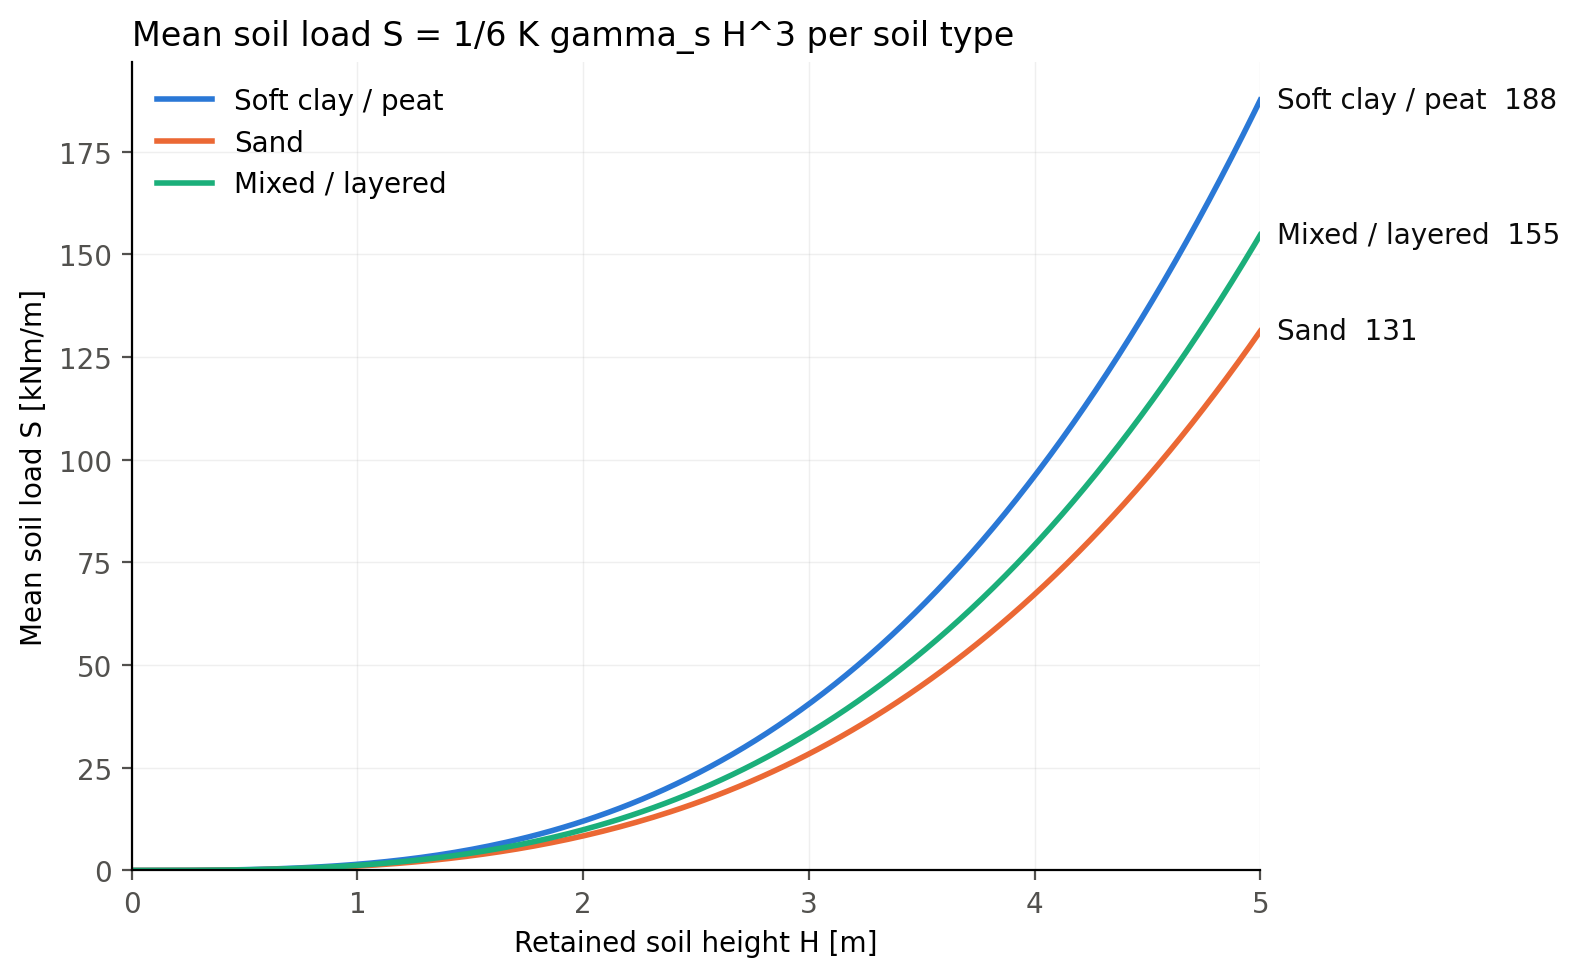
\includegraphics[width=\linewidth]{figures/soil_load_vs_height.png}
        \caption{Soil load versus height}
        \label{fig:soil_load_vs_height}
    \end{subfigure}
    \hfill
    \begin{subfigure}[b]{0.59\linewidth}
        \centering
        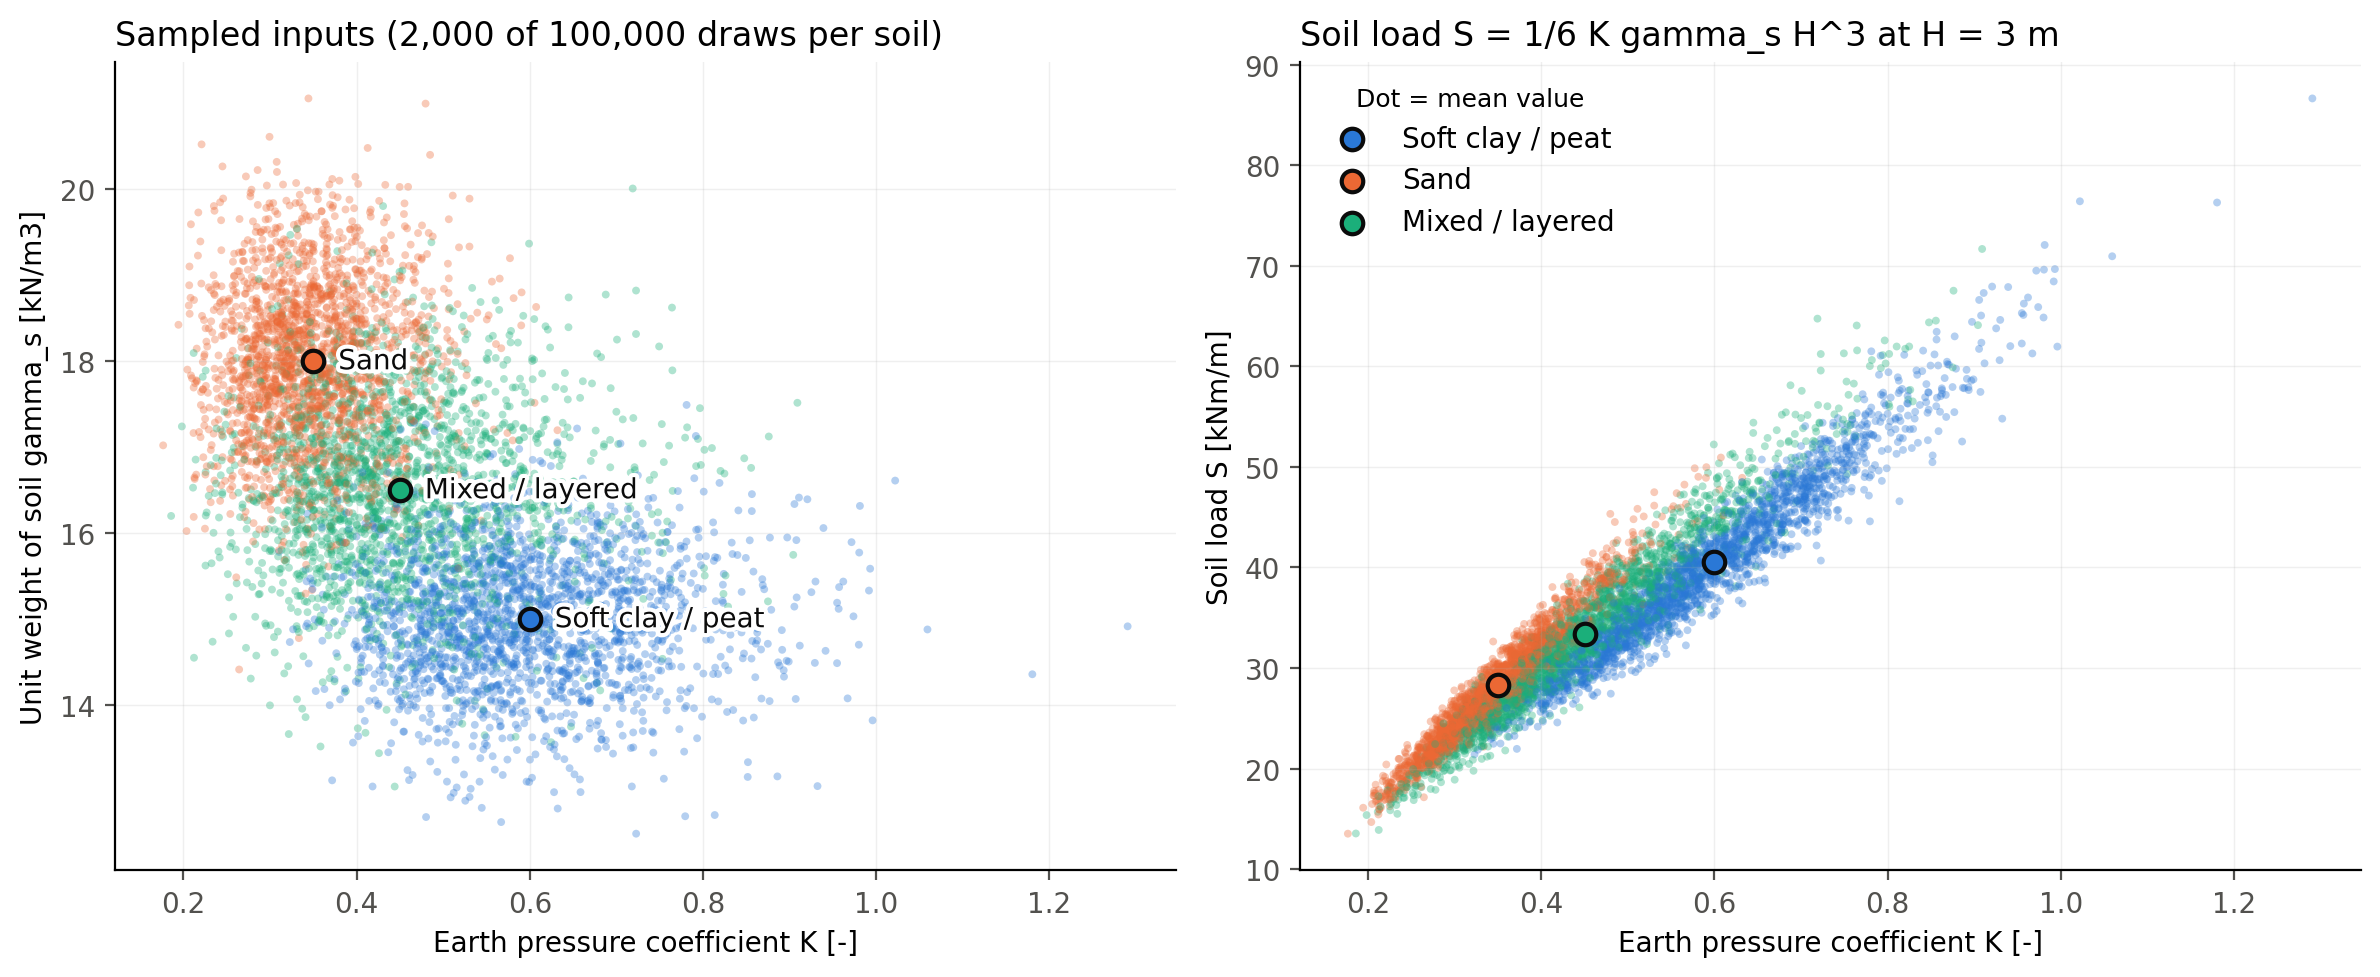
\includegraphics[width=\linewidth]{figures/soil_monte_carlo_scatter.png}
        \caption{Monte Carlo scatter}
        \label{fig:soil_monte_carlo_scatter}
    \end{subfigure}
    \caption{Overall caption for both figures}
    \label{fig:soil_results}
\end{figure}

\subsection{Traffic load on the quay wall}

\textbf{Stress vs moment.} Traffic on the road surface creates a horizontal pressure on the wall (kPa). Integrated over the height it becomes a force (kN/m), and multiplied by its lever arm it becomes the moment (kNm/m) that enters the limit states.

\begin{table}[h]
\centering
\begin{tabular}{@{}llll@{}}
\toprule
 & Stress & Force & Moment \\
\midrule
Expression & $K\,q_{eff}$ & $K\,q_{eff}\,H$ & $S_q=\tfrac{1}{2}\,K\,q_{eff}\,H^2$ \\
Units & kPa & kN/m & kNm/m \\
\bottomrule
\end{tabular}
\end{table}

The pressure is uniform with depth, so the force acts at $H/2$. That is why traffic scales with $H^2$, while soil self-weight (triangular pressure) scales with $H^3$.

\begin{equation}
S_q=\tfrac{1}{2}\,K\,q_{eff}\,H^2
\end{equation}

\textbf{Parameters}
\begin{itemize}
\item $K$: lateral earth pressure coefficient set by soil type
\item $H$: retained height (m).
\item $q_{eff}$: traffic surcharge (kPa), the maximum in the reference period from the ADT-based extreme-value distribution.

\end{itemize}

\textbf{Traffic dependence.} Traffic load $q$ is determined through ADT (heavy-vehicle share, vehicle weights)


\begin{figure}[htp]
    \centering
    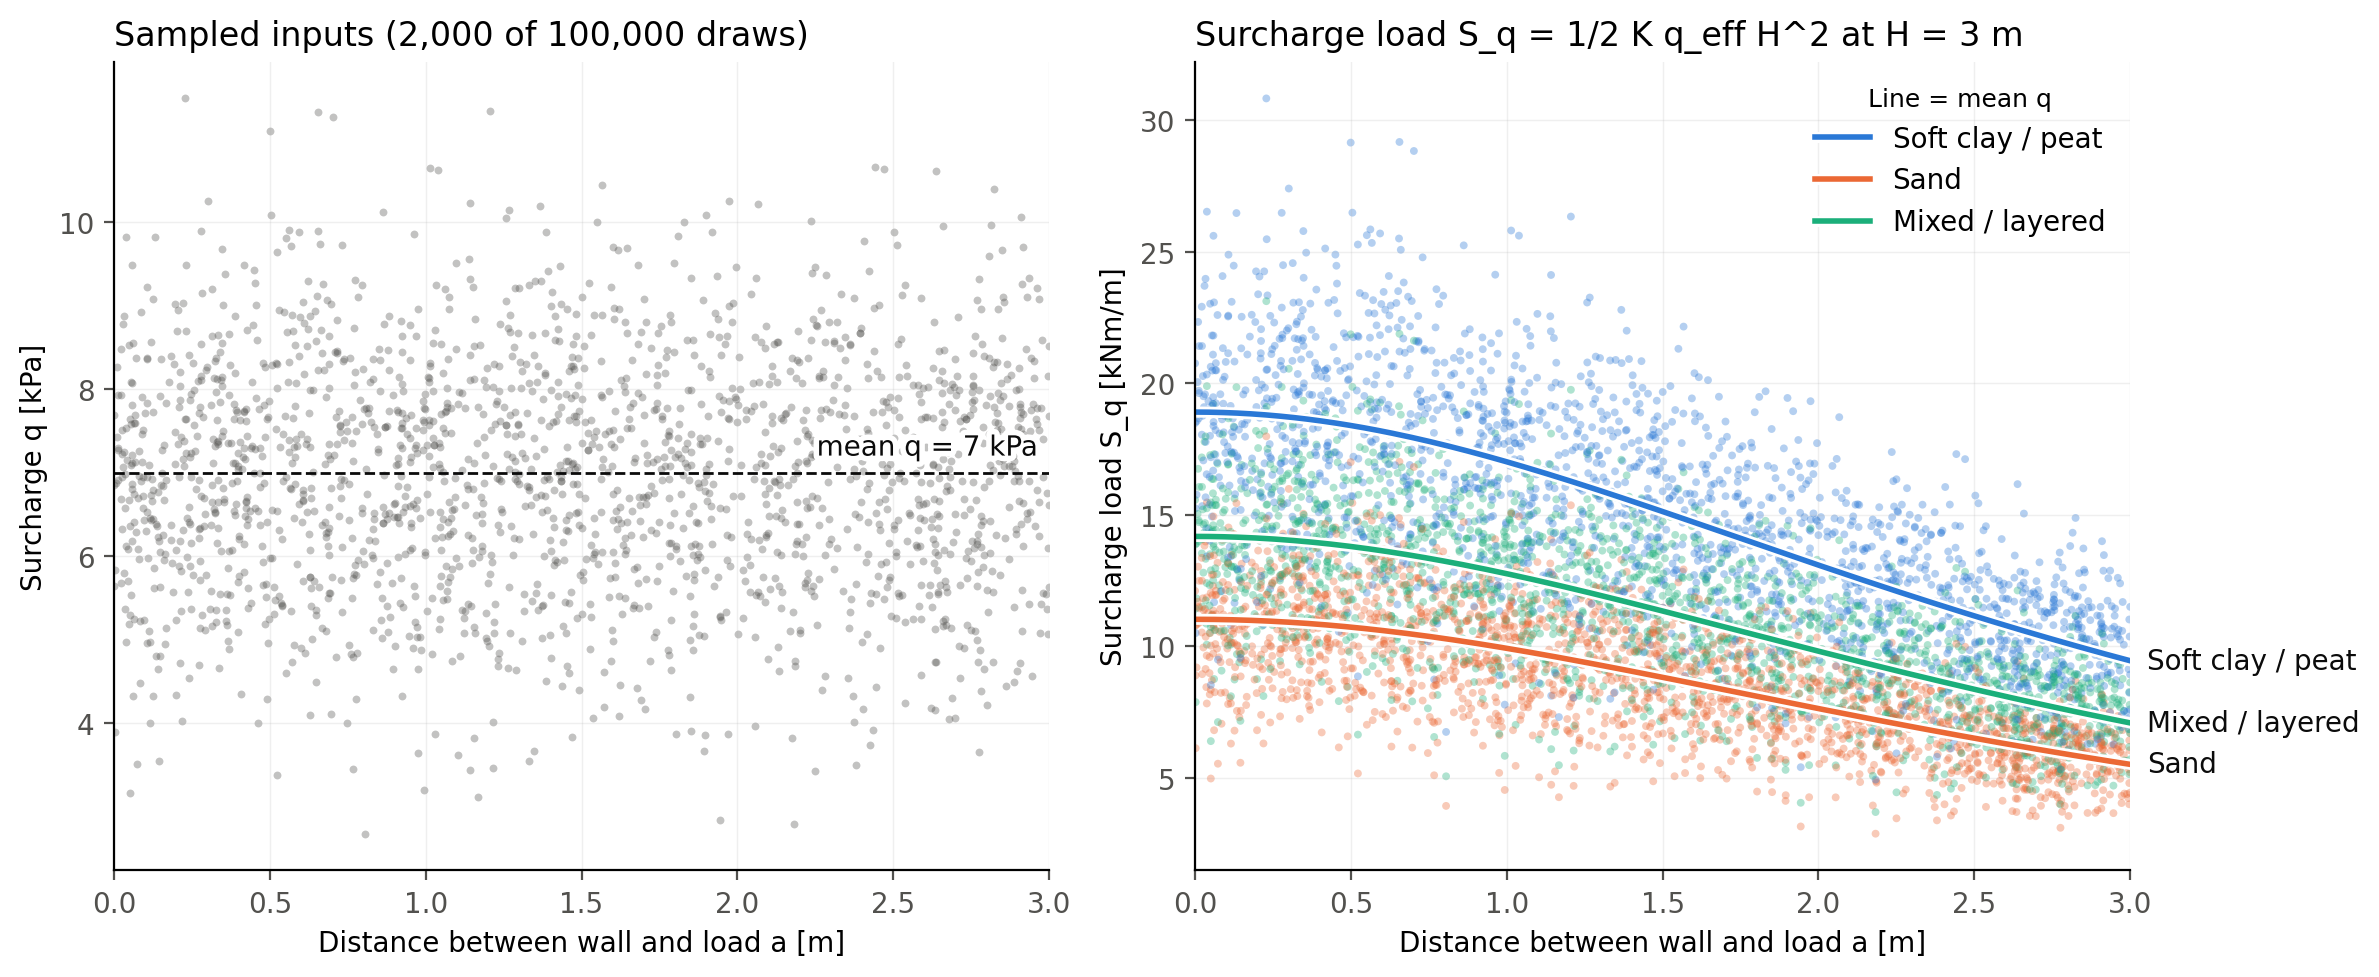
\includegraphics[width=1\linewidth]{figures/surcharge_monte_carlo_scatter.png}
    \caption{Enter Caption}
    \label{fig:placeholder}
\end{figure}




\subsection{Strength of the Quay Wall}

The wall resistance is estimated by its stabilising moment from self-weight to be compared with the overturning moment. A probabilistic approach accounts for uncertainty in age, maintenance, and deterioration.

\textbf{Resistance Moment Formula}

Assuming a rectangular masonry wall, the resisting moment per metre length is:

\begin{equation}
M_{R,0} = \frac{\gamma_m H t^2}{2}
\qquad [\mathrm{kNm/m}]
\end{equation}

where:
\begin{itemize}
    \item $\gamma_m$ is the masonry unit weight ($\mathrm{kN/m^3}$)
    \item $H$ is the effective wall height (m), determined from asset records
    \item $t$ is the effective rectangular wall thickness (m)
\end{itemize}

The formula assumes a uniform rectangular cross-section, constant material unit weight and a moment reference at the wall toe based on wall self-weight.

\textbf{Probability Measure}

A resistance model-uncertainty factor, $\theta_R$, will be included to account for uncertainties that attribute to reduction in resistance.
\begin{equation}
M_R = \theta_R M_{R,0}
\end{equation}

To account for reduction in the wall's effective resistance over time, the following factors inform the assessment:

\begin{itemize}
    \item \textbf{Age:} Time since construction may indicate greater exposure to deterioration and thus loss in resistance loads and moment.

    \item \textbf{Prior maintenance:} Documented repairs, replacement or strengthening  influence the current condition.

    \item \textbf{Foundation type:} Distinguish shallow foundations from piled foundations which affects the governing stability mechanism and support conditions. Unknown foundations are an uncertainty requiring justified assumptions based on data.
    
    \item \textbf{Displacement:} Observed movement affects a quay wall's resistance by indicating possible changes in geometry, foundation support, soil conditions or structural integrity.
    
\end{itemize}


\subsection{Strength of the quay wall foundation}
\label{sec:strength}

The strength $R$ is the moment about the base of the wall that the timber
pile foundation can resist. It has the same unit as the soil, traffic and
tree loads [kNm/m], so that strength and load can be compared directly in
the combined calculation.

\subsubsection*{Step 1: Strength at construction}
No design calculations or pile data are available for the walls in the
Wervengebied. We therefore assume that a wall met the safety level of its
time when it was built. The strength at construction is linked to the load
the wall was designed for:
\begin{equation}
  R_0 = SF_0\,S_d \qquad [\mathrm{kNm/m}], \label{eq:strength_initial}
\end{equation}
where
\begin{itemize}
  \item $R_0$ is the strength of the foundation at construction [kNm/m];
  \item $SF_0$ is the original safety margin [--]. It is lognormal with
        $V = 0.20$. Its mean follows from the calibration in Step~2;
  \item $S_d$ is the design load moment [kNm/m]. It is the soil load
        $S$ (Eq.~\ref{eq:soil_load}) plus the traffic load for a
        surcharge of 5\,kN/m$^2$ on the wharf, without a tree. It is
        computed with the same soil parameters as the load side
        (Table~\ref{tab:soil_distributions}).
\end{itemize}

\subsubsection*{Step 2: Calibration of the safety margin}
The mean of $SF_0$ is chosen so that a new wall had a reliability index
$\beta_0$:
\begin{equation}
  P\bigl(SF_0\,S_d < S_0\bigr) = \Phi(-\beta_0), \label{eq:strength_calibration}
\end{equation}
where
\begin{itemize}
  \item $S_0$ is the load on the new wall [kNm/m]: soil load plus a
        surcharge of 5\,kN/m$^2$, with its annual maximum drawn at random,
        and no tree;
  \item $\Phi$ is the standard normal distribution function;
  \item $\beta_0 = 3.3$ is the target reliability index for a new structure
        [--] \parencite{nen_en1990}.
\end{itemize}
In practice, the mean of $SF_0$ is increased in small steps in a Monte Carlo
simulation until the share of failures for a new wall equals
$\Phi(-3.3) \approx 5\cdot10^{-4}$.

\subsubsection*{Step 3: Decay of the timber piles}
The piles lose diameter in time through bacterial decay. The diameter is
assumed to decrease linearly in time \parencite{sharma2023, klaassen2009}:
\begin{equation}
  D(t) = D_0 - r_b\,t \qquad [\mathrm{m}], \label{eq:pile_diameter}
\end{equation}
where
\begin{itemize}
  \item $D(t)$ is the pile diameter after $t$ years [m];
  \item $D_0$ is the pile diameter at construction [m]. It is normal with
        $\mu = 0.20$\,m and $V = 0.15$. Amsterdam quay walls had pile
        diameters of 200--260\,mm at construction \parencite{sharma2023}, and
        piles of 15--20\,cm were found along the Oudegracht
        \parencite{erfgoed156};
  \item $r_b$ is the decay rate of the pile diameter [m/year]. It is
        lognormal with $\mu = 0.34$\,mm/year and $V = 0.46$
        \parencite{hemel2024}. For pine piles, as in the Oudegracht, rates
        up to 0.50\,mm/year are reported \parencite{klaassen2009};
  \item $t$ is the age of the foundation [years], taken as 2026 minus the
        construction year from the asset file of the municipality.
\end{itemize}

\subsubsection*{Step 4: Strength after $t$ years}
The bending capacity of a round pile is proportional to $D^3$
\parencite{verruijt2018}. The strength after $t$ years is therefore
\begin{equation}
  R(t) = R_0 \left(\frac{D(t)}{D_0}\right)^{3}
         \qquad [\mathrm{kNm/m}], \label{eq:strength_t}
\end{equation}
where $R_0$ follows from Step~1 and $D(t)$ and $D_0$ from Step~3. The factor
$(D(t)/D_0)^3$ lies between 0 and 1 and shows which part of the original
strength is left. $R(t)$ is the strength that is used in the combined
calculation.

\subsubsection*{Step 5: Strength used in the limit state}
The strength of the section in year $t$ is
\begin{equation}
  F_{strength} = R(t) \qquad [\mathrm{kNm/m}], \label{eq:F_strength}
\end{equation}
with $R(t)$ from Eq.~\ref{eq:strength_t}. The load on the section is the sum
of the soil, traffic and tree load moments:
\begin{equation}
  F_{stress} = S + S_{tr} + S_t \qquad [\mathrm{kNm/m}], \label{eq:F_stress}
\end{equation}
where $S$ is the soil load (Eq.~\ref{eq:soil_load}), $S_{tr}$ the traffic
load and $S_t$ the tree load, all as moments about the base. The wall fails
when the load exceeds the strength:
\begin{equation}
  Z = F_{strength} - F_{stress}, \qquad \text{failure when } Z < 0.
  \label{eq:Z}
\end{equation}
Both terms are moments about the base of the wall [kNm/m], so they can be
subtracted directly. The failure probability follows from a Monte Carlo
simulation in which all random variables of the strength and the loads are
drawn together.

\begin{table}[htbp]
  \centering
  \small
  \caption{Strength parameters ($\mu$ = mean, $V$ = coefficient of
           variation).}
  \label{tab:strength_distributions}
  \begin{tabular}{@{}llccp{4.2cm}@{}}
    \toprule
    Symbol & Distribution & $\mu$ & $V$ & Source \\
    \midrule
    $SF_0$ [--]     & lognormal     & calibrated & 0.20 & Eq.~\ref{eq:strength_calibration} \\
    $\beta_0$ [--]  & deterministic & 3.3  & --   & \textcite{nen_en1990} \\
    $D_0$ [m]       & normal        & 0.20 & 0.15 & \textcite{sharma2023}; \textcite{erfgoed156} \\
    $r_b$ [mm/year] & lognormal     & 0.34 & 0.46 & \textcite{hemel2024}; \textcite{klaassen2009} \\
    $t$ [years]     & per section   & --   & --   & asset file (construction year) \\
    \bottomrule
  \end{tabular}
\end{table}



\section{Proposed Scoring Framework for Utrecht's Wervengebied Quay Walls}

The scoring system is used to determine the relative impact of quay-wall failure by assessing factors associated with the surrounding environment, structural condition indicators and maintenance history. Each factor is assigned a score and weighted according to its proposed contribution to the assessment. The combined score provides a consistent basis for comparing quay walls and identifying those requiring further investigation. When considered alongside the probability of failure, the impact assessment informs the overall risk analysis and supports the categorisation and prioritisation of walls for maintenance.


The framework uses five variables: traffic intensity, land use, observed movement, maintenance history and age. All variables use a common scale of 1–5, where 1 represents lower concern and 5 represents higher concern. The method follows the ARK principle of scoring relevant factors and combining them through weighting to support impact determination and risk assessment.

\subsection{Variable Definitions and Scoring Criteria}

\subsubsection{Traffic Intensity}

Traffic intensity represents traffic-related surcharge and repeated loading behind the quay wall. It is assessed using Utrecht's open municipal dataset of modelled average working-day traffic. The 24-hour total, expressed as vehicles per average working day, is used for consistent comparison.

\begin{table}[htbp]
    \centering
    \caption{Scoring criteria for traffic intensity}
    \vspace{2mm}
    \begin{tabularx}{\textwidth}{c X X}
        \toprule
        \textbf{Score} & \textbf{Average working-day traffic (vehicles/day)} & \textbf{Interpretation} \\
        \midrule
        1 & Below 500 & Very low motor-traffic exposure \\
        2 & 500–1,999 & Low traffic \\
        3 & 2,000–4,999 & Moderate traffic \\
        4 & 5,000–9,999 & High traffic \\
        5 & 10,000 or more & Very high traffic exposure \\
        \bottomrule
    \end{tabularx}
\end{table}

Traffic volume is an important indicator for screening traffic-related surcharge, although it does not directly quantify axle loads or the actual surcharge acting on the wall.

\subsubsection{Land Use}

Land use captures the intensity and functional importance of activities behind the wall. It indicates the potential exposure and consequences of failure. Utrecht's official planning and land-use information can be used to classify the adjoining area.

\begin{table}[htbp]
    \centering
    \caption{Scoring criteria for land use}
    \vspace{2mm}
    \begin{tabularx}{\textwidth}{c X X}
        \toprule
        \textbf{Score} & \textbf{Land-use category} & \textbf{Interpretation} \\
        \midrule
        1 & Unoccupied or low-use open space & Limited activity and exposure \\
        2 & Green space or low-intensity recreational use & Occasional users \\
        3 & Residential frontage or local public realm & Regular use by residents and pedestrians \\
        4 & Commercial frontage, hospitality, busy public realm or major pedestrian route & Frequent occupation and activity \\
        5 & Critical access, major public gathering location or highly occupied frontage with substantial consequences of failure & High potential exposure and disruption \\
        \bottomrule
    \end{tabularx}
\end{table}

\subsubsection{Observed Movement}

Movement indicates possible deformation, settlement or loss of support. The Dutch Bodemdalingskaart provides deformation measurements and rates, including satellite-derived and other geodetic observations. The scores below use absolute vertical movement rates.

\begin{table}[htbp]
    \centering
    \caption{Scoring criteria for observed movement}
    \vspace{2mm}
    \begin{tabularx}{\textwidth}{c X X}
        \toprule
        \textbf{Score} & \textbf{Absolute vertical movement rate} & \textbf{Interpretation} \\
        \midrule
        1 & Below 1 mm/year & Low measured movement \\
        2 & 1 to below 2 mm/year & Limited movement \\
        3 & 2 to below 3 mm/year & Moderate movement \\
        4 & 3–5 mm/year & High movement \\
        5 & Above 5 mm/year & Very high movement \\
        \bottomrule
    \end{tabularx}
\end{table}

\subsubsection{Maintenance History}

Maintenance history reflects the time since the last verified substantive structural intervention and whether the intervention addressed the relevant failure mechanism. The assessment draws on the municipal asset inventory and the Werven programme's records of completed and planned repairs.

\begin{table}[htbp]
    \centering
    \caption{Scoring criteria for maintenance history}
    \vspace{2mm}
    \begin{tabularx}{\textwidth}{c X X}
        \toprule
        \textbf{Score} & \textbf{Time since last verified substantive structural maintenance} & \textbf{Interpretation} \\
        \midrule
        1 & 0–10 years & Recent intervention \\
        2 & More than 10–20 years & Relatively recent intervention \\
        3 & More than 20–30 years & Intermediate period since intervention \\
        4 & More than 30–50 years & Long period since intervention \\
        5 & More than 50 years, or no maintenance history found & Very long period or unknown history \\
        \bottomrule
    \end{tabularx}
\end{table}

\subsubsection{Age}

Age is calculated from the recorded construction year, using 2026 as the assessment year. The bands distinguish newer structures from older historic assets.

\begin{table}[htbp]
    \centering
    \caption{Scoring criteria for age}
    \vspace{2mm}
    \begin{tabularx}{\textwidth}{c X X}
        \toprule
        \textbf{Score} & \textbf{Age in 2026} & \textbf{Interpretation} \\
        \midrule
        1 & 0–50 years & Relatively young \\
        2 & 50–100 years & Moderate age \\
        3 & 100–150 years & Older structure \\
        4 & 150–200 years & Very old structure \\
        5 & More than 200 years & Historic \\
        \bottomrule
    \end{tabularx}
\end{table}

\subsection{Weighted Scoring Table}

The proposed weights provide a consistent way to combine the variables while reflecting their different roles in the assessment. Observed movement receives a higher weight because it provides measurable evidence of possible deformation or settlement. Maintenance history and age help characterise the wall's history and potential exposure to deterioration, while traffic intensity and land use represent loading conditions and the surrounding environment. The weights remain initial assumptions and should be reviewed through sensitivity analysis and municipal prioritisation of factors.

\begin{table}[htbp]
    \centering
    \caption{Weighted scoring summary}
    \vspace{2mm}
    \begin{tabularx}{\textwidth}{X X c c X}
        \toprule
        \textbf{Variable} & \textbf{Value recorded for each wall} & \textbf{Score} & \textbf{Weight (\%)} & \textbf{Score $\times$ weight} \\
        \midrule
        Traffic intensity & Average workday vehicles/day & 1–5 & 15 & Score $\times$ 15 \\
        Land use & Adjacent land-use category & 1–5 & 10 & Score $\times$ 10 \\
        Observed movement & Verified movement rate (mm/year) & 1–5 & 25 & Score $\times$ 25 \\
        Maintenance history & Years since completed structural intervention & 1–5 & 15 & Score $\times$ 15 \\
        Age & Years since construction or substantial reconstruction & 1–5 & 10 & Score $\times$ 10 \\
        \midrule
        \textbf{Total} & & & \textbf{100} & \textbf{Sum of weighted contributions} \\
        \bottomrule
    \end{tabularx}
\end{table}

The final index is calculated by dividing the sum of weighted contributions by the total weight. The resulting index can then be used to rank walls for further investigation and considered alongside the probability of failure in the overall risk assessment.


